\documentclass{cskkuproject}

% ==========================================
% ข้อมูลโครงงาน — กรอกข้อมูลที่นี่
% ==========================================

\titleTH{ระบบจำแนกและวิเคราะห์ข่าวสารอัตโนมัติด้วยเทคนิคการประมวลผล ภาษาธรรมชาติแบบเฉพาะประเภท}
\titleEN{Category-Specific News Classification and NLP Analytics Pipeline}

% ข้อมูลนักศึกษาคนที่ 1 (กรอกข้อมูลจริงก่อนส่ง)
\firstStudentID{663380214-4}
\firstStudentPrefixTH{นาย}
\firstStudentPrefixEN{Mr.}
\firstStudentNameTH{นราวิชญ์ ศิริพล}
\firstStudentNameEN{Narawit Siripol}

% ข้อมูลนักศึกษาคนที่ 2
% *** ถ้าทำโครงงานคนเดียว ให้เว้นว่างไว้ทั้งหมด (เหมือนด้านล่าง) ***
% *** ถ้ามี 2 คน ให้กรอกข้อมูลเหมือนคนที่ 1 ***
\secondStudentID{663380028-1}
\secondStudentPrefixTH{นาย}
\secondStudentPrefixEN{Mr.}
\secondStudentNameTH{อัสดาวุฒิ เอื้อวงค์}
\secondStudentNameEN{Ausadawut Aueawong}

% ข้อมูลหลักสูตร
\degreeTH{วิทยาศาสตรบัณฑิต}
\degreeEN{Bachelor of Science}
\majorTH{วิทยาการคอมพิวเตอร์}
\majorEN{Computer Science}

% อาจารย์ที่ปรึกษา (กรอกข้อมูลจริงก่อนส่ง)
\advisorTH{อ.ดร.พบพร ด่านวิรุทัย}
\advisorEN{Dr. Pobporn Danvirutai}

% ปีการศึกษา
\academicYearTH{2569}
\academicYearEN{2026}

% รหัสวิชา (CP354 771 = โครงงาน 1, CP354 772 = โครงงาน 2)
\courseCode{CP354 771}
\courseName{โครงงานคอมพิวเตอร์ 1}
\semester{1}

% คำสำคัญ
\keywordsTH{การจำแนกข่าว, การวิเคราะห์ข้อความ, การประมวลผลภาษาธรรมชาติ, เว็บสแครปปิง, โมเดลภาษาขนาดใหญ่, อัลกอริทึมแนะนำข่าว}
\keywordsEN{News classification, Text analytics, Natural language processing, Web scraping, Large language model, Recommendation algorithm}


\begin{document}

% ==========================================
% หน้าปก
% ==========================================
% คำสั่งด้านล่างสร้างหน้าปกอัตโนมัติจากข้อมูลที่กรอกด้านบน
% ไม่ต้องแก้ไขส่วนนี้
\maketitlepage

% ตั้งค่าเลขหน้าส่วนต้นเป็นอักษรไทย (ก, ข, ค, ...)
\pagenumbering{arabic}
\setcounter{page}{0}
\renewcommand{\thepage}{\ThaiAlph{\value{page}}}

% ==========================================
% บทคัดย่อ
% ==========================================
\begin{abstractTH}
% บทคัดย่อภาษาไทย
% หมายเหตุ: ไม่ควรเกิน 300 คำ
% ควรครอบคลุม: วัตถุประสงค์ → วิธีการ → ผลลัพธ์ → การประยุกต์ใช้

โครงงานนี้มีวัตถุประสงค์เพื่อศึกษาและพัฒนาระบบจำแนกและวิเคราะห์ข่าวสารอัตโนมัติด้วยเทคนิคการประมวลผลภาษาธรรมชาติแบบเฉพาะประเภท (Category-Specific NLP Analytics) โดยระบบพัฒนาด้วยภาษา Python ร่วมกับเฟรมเวิร์ค FastAPI สำหรับส่วน Backend และภาษา JavaScript ร่วมกับ Tailwind CSS และ Socket.IO สำหรับส่วน Frontend ระบบทำการรวบรวมข่าวจากเว็บไซต์ข่าวไทยด้วยเทคนิคเว็บสแครปปิง การอ่าน RSS Feed และการจำลองเบราว์เซอร์ด้วย Playwright จากนั้นส่งเนื้อหาข่าวในรูปแบบ Markdown ไปยังโมเดลภาษาขนาดใหญ่ผ่านบริการ KKU Gen.AI เพื่อสร้างบทสรุป ประเด็นสำคัญ อารมณ์ของข่าว และคำสำคัญในภาษาเดียวกับต้นฉบับ พร้อมจำแนกหมวดหมู่ข่าวออกเป็นหมวดหมู่เฉพาะทางด้วยการตัดคำภาษาไทยด้วย PyThaiNLP ร่วมกับกฎคำสำคัญและโมเดล SVM และแสดงผลข่าวพร้อมสรุปบนเว็บแอปพลิเคชันแบบเรียลไทม์ผ่าน WebSocket ระบบยังมีกลไกการจัดการแคชและคุกกี้เพื่อปรับแต่งประสบการณ์ผู้ใช้และป้อนข้อมูลให้อัลกอริทึมแนะนำข่าว โครงงานนี้เป็นประโยชน์ต่อการลดภาระของผู้อ่านในการติดตามข่าวจากหลายเว็บไซต์ และเป็นแนวทางในการประยุกต์ใช้เทคนิค NLP และโมเดลภาษาขนาดใหญ่สำหรับการวิเคราะห์ข่าวสารอัตโนมัติ
\end{abstractTH}

\begin{abstractEN}
% ABSTRACT (English)
% Note: Should not exceed 300 words.
% Should cover: Objective, Methodology, Results, Applications
% Use Past tense for objectives and methodology
% Use Present tense for results and applications

This project aims to study and develop a Category-Specific News Classification and NLP Analytics Pipeline for automatic news processing. The system is developed with Python and the FastAPI framework for the backend, and JavaScript with Tailwind CSS and Socket.IO for the frontend. News articles are collected from Thai news websites using web scraping, RSS feed parsing, and Playwright browser automation for JavaScript-rendered pages. The collected article content in Markdown format is then sent to a large language model through the KKU Gen.AI service to generate a summary, key points, sentiment, and keywords in the same language as the original article. The system also classifies news into specific categories using Thai word segmentation with PyThaiNLP combined with keyword-based rules and a Support Vector Machine model, and presents the news with summaries on a web application in real time through WebSocket. Additionally, the system incorporates a cache and cookie management mechanism — including personalize cookies for user preferences and algorithm cookies for tracking reading behavior — to feed a recommendation algorithm that tailors news delivery to individual users. This project is beneficial for reducing the effort of readers who need to follow news across multiple websites, and serves as a guideline for applying NLP techniques and large language models to automatic news analytics.
\end{abstractEN}

% ==========================================
% กิตติกรรมประกาศ
% ==========================================
\begin{acknowledgement}
% กิตติกรรมประกาศ
% หมายเหตุ: ไม่เกิน 1 หน้ากระดาษ
%
% *** ลบข้อความตัวอย่างด้านล่าง แล้วเขียนกิตติกรรมประกาศของตนเอง ***

ข้าพเจ้าขอขอบพระคุณ อ.ดร.พบพร ด่านวิรุทัย อาจารย์ที่ปรึกษาโครงงาน
ที่ได้กรุณาให้คำแนะนำ คำปรึกษา และข้อเสนอแนะอันเป็นประโยชน์
ตลอดระยะเวลาการดำเนินโครงงานฉบับนี้
รวมทั้งสละเวลาในการตรวจแก้ไขและให้กำลังใจ
จนทำให้โครงงานนี้สำเร็จลุล่วงไปได้ด้วยดี

ขอขอบพระคุณคณาจารย์ในสาขาวิชาวิทยาการคอมพิวเตอร์
วิทยาลัยการคอมพิวเตอร์ มหาวิทยาลัยขอนแก่น
ทุกท่านที่ได้ถ่ายทอดความรู้ทางวิชาการ
ซึ่งเป็นพื้นฐานสำคัญในการศึกษาค้นคว้าและจัดทำโครงงานนี้

ขอขอบพระคุณเพื่อนร่วมชั้นและผู้ที่เกี่ยวข้องทุกท่าน
ที่ได้ให้ความช่วยเหลือ แนะนำ และแลกเปลี่ยนความคิดเห็น
ซึ่งเป็นประโยชน์ต่อการดำเนินงานในหลายด้าน

ท้ายที่สุดนี้ ข้าพเจ้าขอขอบพระคุณบิดา มารดา และครอบครัว
ที่ให้การสนับสนุน ส่งเสริม และเป็นกำลังใจ
ตลอดระยะเวลาของการศึกษา

\end{acknowledgement}

% ==========================================
% สารบัญ
% ==========================================
\tableofcontents
\clearpage
\listoffigures
\clearpage
\listoftables
\clearpage

% ==========================================
% สัญลักษณ์และคำย่อ (ถ้ามี — uncomment ด้านล่าง)
% ==========================================
% \begin{symbolpage}
% \input{symbols}
% \end{symbolpage}

% ==========================================
% เนื้อเรื่อง 5 บท
% ==========================================
% เริ่มนับเลขหน้าใหม่เป็นเลขอารบิก (1, 2, 3, ...)
% ไม่ต้องแก้ไขส่วนนี้
\pagenumbering{arabic}
\setcounter{page}{1}

\chapterone
\chaptertwo
\chapterthree

% ==========================================
% ข้อเสนอโครงงาน (Proposal) — นำเสนอถึงบทที่ 3
% บทที่ 4 และ 5 เป็นการวิเคราะห์/พัฒนาระบบและสรุปผล
% จะเขียนในรายงานฉบับสมบูรณ์
% *** ถ้าต้องการแสดงในไฟล์ ให้ uncomment สองบรรทัดด้านล่าง ***
% ==========================================
% \chapterfour
% \chapterfive

% ==========================================
% เอกสารอ้างอิง
% ==========================================
% *** ไม่ต้องแก้ไขส่วนนี้ ***
% ระบบจะดึงรายการอ้างอิงจากไฟล์ references.bib อัตโนมัติ
% ให้แก้ไขรายการอ้างอิงในไฟล์ references.bib แทน
\clearpage
\addcontentsline{toc}{chapter}{เอกสารอ้างอิง}
\makeatletter
\let\ps@plain\ps@empty
\makeatother
\bibliographystyle{ieeetr}
\bibliography{references}

% ==========================================
% ภาคผนวก
% ==========================================
% =============================
% ภาคผนวก
% =============================
% หมายเหตุ: ก่อนเริ่มภาคผนวก ระบบจะสร้างหน้าคั่นให้อัตโนมัติ
% ใช้คำสั่ง \appendiceschapter{ชื่อภาคผนวก} สำหรับแต่ละภาคผนวก
% ระบบจะกำหนดตัวอักษร ก, ข, ค ... ให้โดยอัตโนมัติ
%
% *** ลบข้อความตัวอย่างด้านล่าง แล้วใส่ภาพ UI / Prototype ของตนเอง ***

% =============================
% ภาคผนวก ก
% =============================
\setcounter{chapter}{-1}
\appendiceschapter{ตัวอย่าง UI หรือ Prototype}

\section*{ภาพหน้าจอระบบ}

ภาคผนวกนี้แสดงตัวอย่างหน้าจอของระบบที่พัฒนาขึ้น เพื่อให้เห็นภาพรวมของการออกแบบส่วนติดต่อกับผู้ใช้

หน้าจอเข้าสู่ระบบ (Login) แสดงดังภาพที่ \ref{fig:ui_login}

% *** เปลี่ยนชื่อไฟล์จาก ui-login.png เป็นชื่อไฟล์ของคุณ ***
\begin{figure}[H]
\centering
% 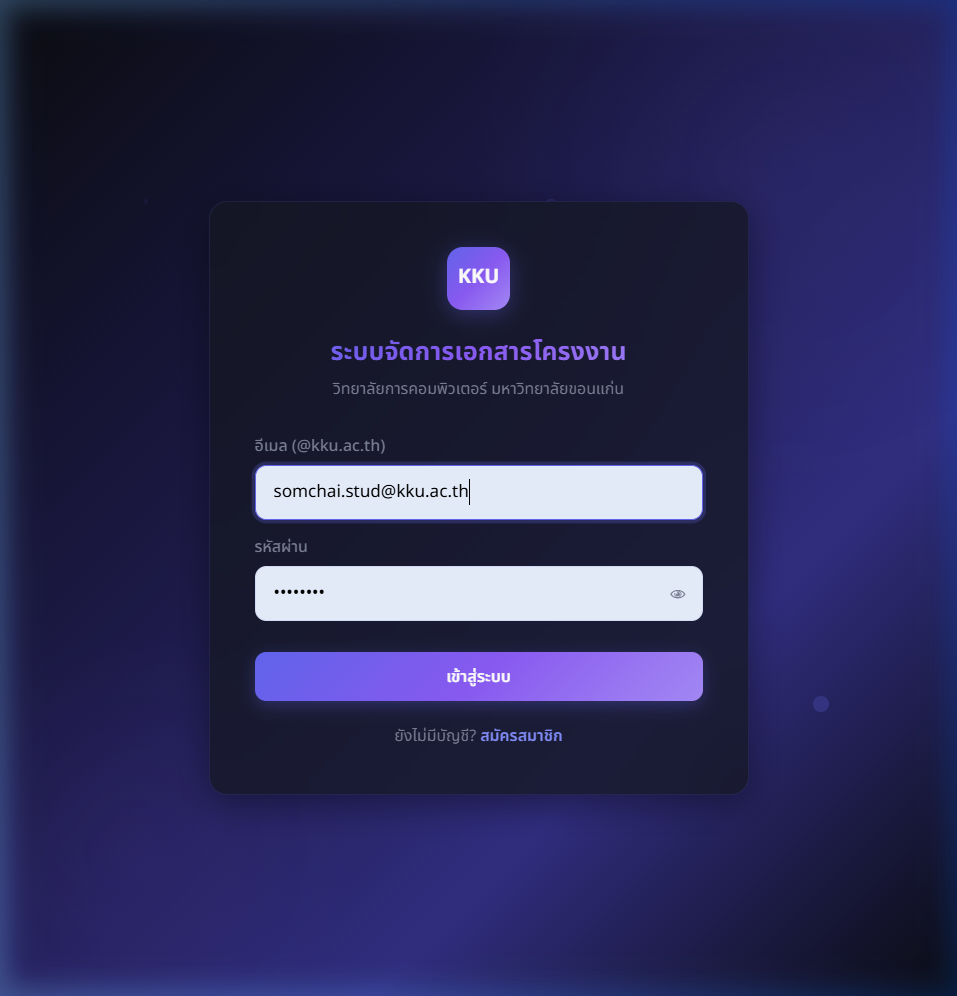
\includegraphics[width=0.8\textwidth]{images/ui-login.png}
\fbox{\parbox{0.75\textwidth}{\centering\vspace{4cm}\textit{แทรกภาพหน้าจอ Login ที่นี่}\\ใช้คำสั่ง \texttt{\textbackslash includegraphics}\vspace{4cm}}}
\caption{หน้าจอเข้าสู่ระบบ (Login)}
\label{fig:ui_login}
\end{figure}

หน้าจอหลัก (Dashboard) แสดงดังภาพที่ \ref{fig:ui_dashboard}

\begin{figure}[H]
\centering
% 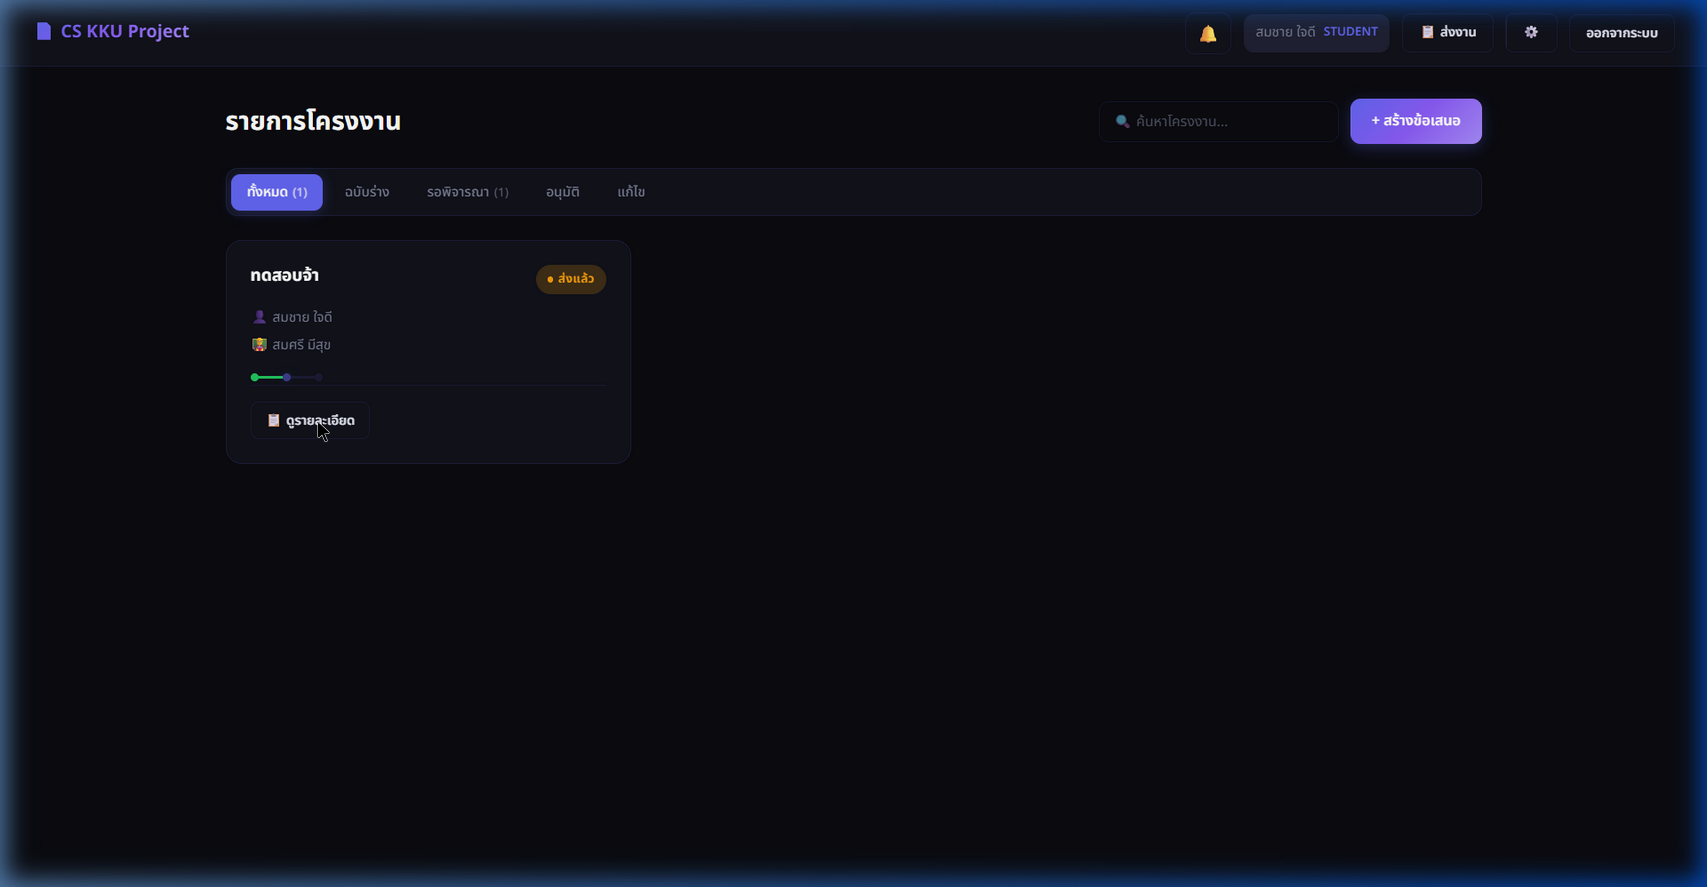
\includegraphics[width=0.8\textwidth]{images/ui-dashboard.png}
\fbox{\parbox{0.75\textwidth}{\centering\vspace{4cm}\textit{แทรกภาพหน้าจอหลักที่นี่}\vspace{4cm}}}
\caption{หน้าจอหลัก (Dashboard)}
\label{fig:ui_dashboard}
\end{figure}

\section*{คู่มือการใช้งาน}

อธิบายขั้นตอนการใช้งานระบบโดยสังเขป\ldots{}

% =============================
% ภาคผนวก ข (ตัวอย่าง — uncomment ถ้าต้องการ)
% =============================
% \appendiceschapter{รายละเอียดเพิ่มเติม}
% \section*{หัวข้อ}
% เนื้อหาภาคผนวก ข


\end{document}
